\chapter{Introduction}
Fitting is the process of optimising the parameters of a 3DMM when a 2D image is given. There are different approaches on how to do that. Some use a mask with labels for each pixel of the image that determine whether or not the pixel represents a part of the imaged face. An additional difficulty is partial occlusion of the facial region, which must be excluded from the mask too. To achieve satisfying fits, the segmentation has to cut out the face as accurately as possible. There are different approaches to algorithmically generate such a mask. Due to the variety and diversity of such occlusions, this is not a simple problem. In this thesis, the quality of such segmentations by machine-learning-algorithms is measured. We compare the neural network of Nirkin er al \cite{nirkin2018_faceswap} and the existing model-based top-down approach by Egger et al \cite{egger_paper}.


\section{Artificial Neural Networks}
The idea of artificial neural networks was somehow influenced by biology. These networks consist of a variety of neurons which are grouped in layers. The way each neuron works is very simple. It takes multiple inputs of varying strength from other neurons, sums them up, puts the sum into a non-linear function (e.g. Maxout, Sigmoid, ReLu) [\Cref{fig:chap1:ActivFunctions}], and decides depending on the output if it should send a stimulus itself and if so, in which strength. Each layer is somehow connected to the next layer. Some layers are fully connected (each neuron of a layer is connected to every other neuron in the next layer) while others are convolutional. Convolutional means that a neuron only gets an input of spatially close neighbours in the previous layer. There are many different architectures which mainly differ in the number of layers, number of neurons per layer, and the interconnectivity of the neurons. A classical convolutional neural network (CNN) is depicted in [Figure \ref{fig:chap1:classicalCNN}].

\begin{figure}[H]
	\centering
	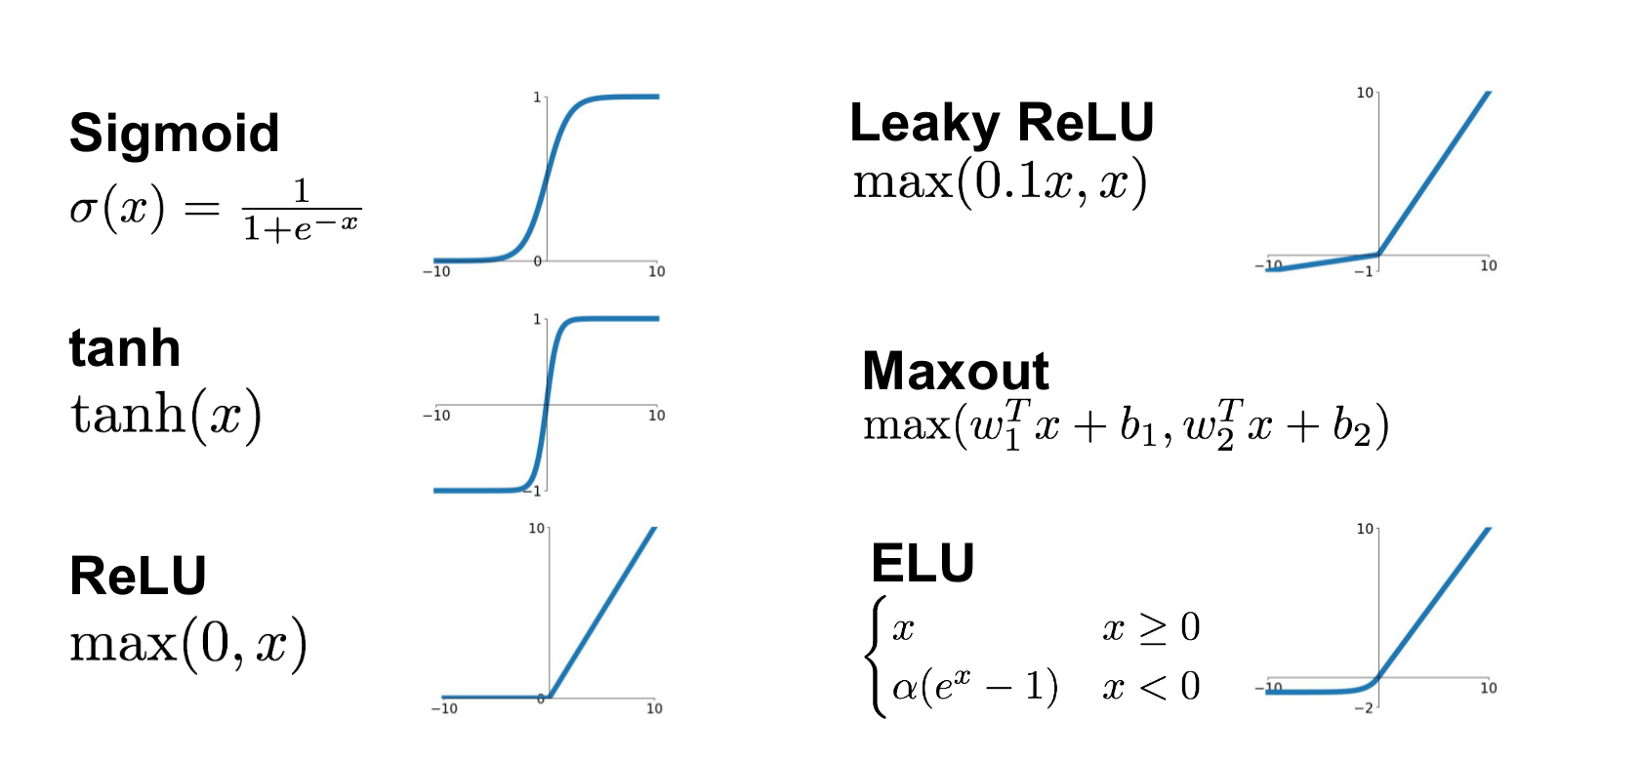
\includegraphics[width=1\linewidth]{Figures/chap1/ActivFunctions.png}
	\caption[Caption for LOF]{Six often used activation functions\footnotemark. The most commonly used activation function is ReLU because of its simplicity. The disadvantage of this function is if one input has a negative sign, then all following neurons output a signal of 0. An improvement of ReLU is Leaky ReLU.}
	\label{fig:chap1:ActivFunctions}
\end{figure}

\footnotetext{Jadon S. (2015 March). Introduction to Different Activation Functions for Deep Learning. Retrieved July 19, 2018 from \textit{https://medium.com/@shrutijadon10104776/survey-on-activation-functions-for-deep-learning-9689331ba092}}

\begin{figure}[H]
	\centering
	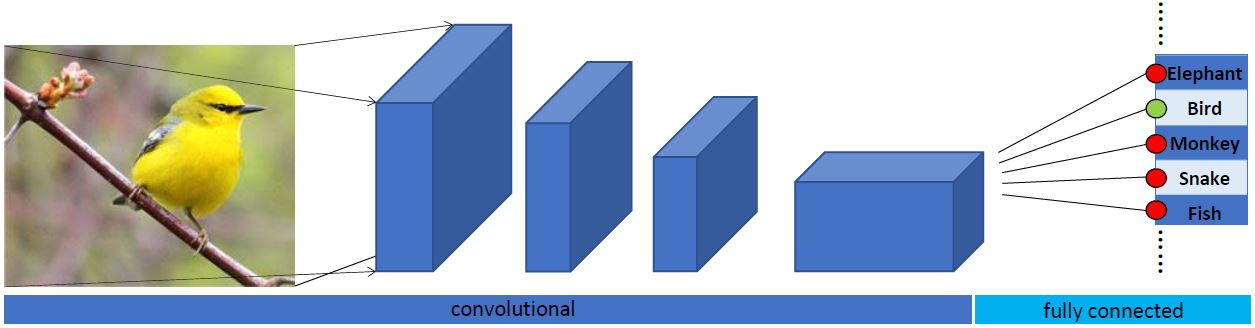
\includegraphics[width=1\linewidth]{Figures/chap1/classicalCNN.JPG}
	\caption{An example of a classical convolutional neural network (CNN). After a certain number of convolutions, a pooling layer extracts the most important information of the image and writes it into the next layer. That is why the picture is getting smaller and smaller until just a vector is left.}
	\label{fig:chap1:classicalCNN}
\end{figure}

Already in 1943, Warren McCulloch and Walter Pitts \cite{mcculloch} showed that even simple networks of this kind can simulate every possible logical formula. For this, they used a neuron model which consisted of simple logic gates and could only process binary input and output signals.

\begin{figure}[H]
	\centering
	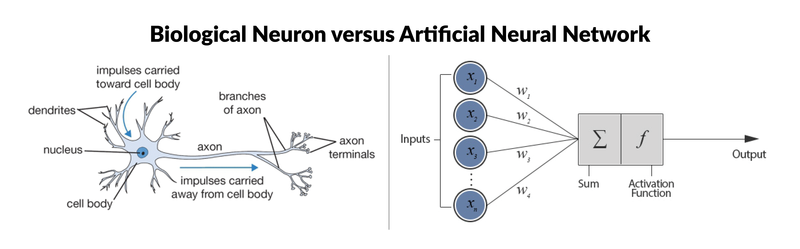
\includegraphics[width=1\linewidth]{Figures/chap1/bio_vs_arti_neuron.png}
	\caption[Caption for LOF]{The left-hand side of the image\footnotemark\ shows a biological neuron. It is a nerve cell which occurs in almost every animal. On the right-hand side, an artificial neuron is depicted. It sums up the stimuli of the previous neurons, applies an activation function to the sum, and forwards the output.}
	\label{fig:test1}
\end{figure}

\footnotetext{Willems K. (2017 May, 2nd). Keras Tutorial: Deep Learning in Python. Retrieved July 10, 2018 from \textit{https://www.datacamp.com/community/tutorials/deep-learning-python}}

\begin{figure}[H]
	\centering
	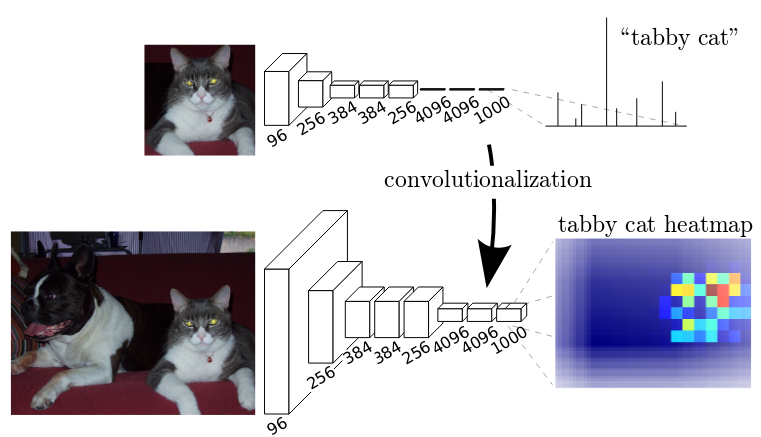
\includegraphics[width=1\linewidth]{Figures/chap1/JLongEtAl.png}
	\caption{The transformation from a CNN into an FCN. This is a schematic diagram of Long et al \cite{jlong}, which fine-tuned the network used in this work. They call this process "convolutionalization". They turn the fully connected layers into convolution layers which produces an efficient machine for end-to-end dense learning. }
	\label{fig:chap1:JLongEtAl}
\end{figure}

\section{The Fully Convolutional Network Used}
\label{sec:theFCN}
For this thesis, a pretrained fully convolutional network from \cite{nirkin2018_faceswap} is used. A fully convolutional network (often called: FCN) is basically a CNN but with a modified architecture. An FCN does not have the fully connected layers which are usually found at the end of an CNN [compare \Cref{fig:chap1:classicalCNN} and \Cref{fig:chap1:JLongEtAl}]. These layers would enable the network to make decisions based on global information. A CNN for example can be used for classification. Nevertheless, for image analysis we want local information of the input image (we do not want to know if there is a face in the image, but where the face is in the image). Therefore, a FCN uses only convolutional and pooling layers. In the whole fully convolutional network only the following structure is repeated: One or more convolution layers and a pooling layer which downsamples the picture. This constellation is recurring several times.\\
\\
The assembly of the network used for this thesis follows the FCN-8s-VGG architecture with extensions of Long et al \cite{jlong} [\Cref{fig:chap1:JLongEtAl}]. The first part 'FCN' stands for 'fully convolutional network', '8s' means that the result gets upsampled eight times (because of the pooling layers), and 'VGG' means that the popular 16-layer network by Oxford's visual geometry group \cite{ksimonyan} is used [\Cref{fig:chap1:VGGnet}]. The original task of the network was to find the name of an object in an input image. The network could distinguish between 1000 different objects. Each cell in the final vector (1*1000 in size) was a boolean variable for one specific item. A schematic representation of this architecture can be found in [\Cref{fig:chap1:classicalCNN}].\\
\\
For our experiments a pretrained fully convolutional network (FCN) of \cite{nirkin2018_faceswap} is used. It was shown that even with a widespread network, good segmentation can be made and that the network does not have to be specially tailored for the future purpose. However, the network must have been trained with a large enough data set. Nirkin et al used the FCN for intra- and inter-subject face swapping on the Labeled Faces in the Wild (LFW) dataset and showed that intra-subject swapped faces remain as recognisable as before the swap and that in the inter-subject version better face swapping  leads to less perceptibility.\\
\\
Nirkin et al used a semi-supervised approach to produce training data in order to train the FCN. To make large quantities of them, 2'043 face videos of the IARPA Janus CS2 dataset of Klare et al \cite{IARPAJanus} were used. To avoid searching for the face in every frame of the video, they used motion queues which tracked the face given an initial segmentation based on the approach of \cite{grundmann} which enriched their training set to 9'818 images. To enlarge the collection of images, they rendered 3D Shapes of various objects (e.g. sunglasses, hands) into existing images. Each occlusion adds 9'500 images to their training set.\\

\begin{figure}[H]
	\centering
	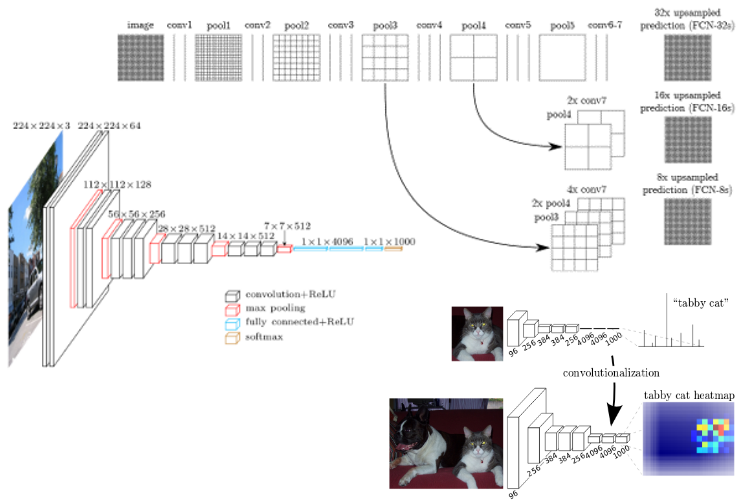
\includegraphics[width=1\linewidth]{Figures/fcn_1.png}
	\caption{In the lower-left corner, the 16 layers of the well known VGGnet are shown. In the top-right, you can see the meaning of the '8s' term of the FCN-name. It means that the resulting image has to be 8x upsampled, to get a replica of it which is equal in size to the input image.}
	\label{fig:chap1:VGGnet}
\end{figure}

\section{Occlusion aware 3DMM}

Egger et al propose a fully automated, probabilistic and occlusion-aware 3D morphable face model adaptation framework \cite{egger_paper}. These methods use an iterative approach to label each pixel whether it belongs to the face or to the background. This approach can handle multiple labels and differentiate between multiple occlusion types, for example, face specific ones (eg. beards) and background. For updating the z-labels they use an algorithm which classifies a pixel based on the probabilities for each possible label, but for our experiments, we limited ourselves to two. We only need to distinguish between the face (including skin and beard) and the background.\\

\pagebreak

The algorithm does two things at the same time. In addition to creating a face mask (segmentation), it estimates the parameters of the popular Basel face Model to reconstruct the given face. It is an EM-algorithm-like method to solve two problems simultaneously. In the E-steps Egger et al update the z-labels and in the M-steps they update the face model  parameters based on the current estimate of the z-labels. For face model adaptation they apply a stochastic sampling strategy based on the Metropolis–Hastings algorithm (Markov Chain Monte Carlo). The likelihood of each pixel is split up into a background model ($X_{BG}$) and a foreground model ($X_{FG}$).
\[ 
\underbrace{p(\Theta |I)=p(I| \Theta)*p(\Theta)}_{\mathclap{\text{\parbox{4.5cm}{posterior probability of face model parameters $\Theta$ given an image $I$}}}}\quad\quad\text{ with: }p(I|\Theta)=\prod_{X \in \text{pixels}}p(X_{BG}|\Theta)^{z-1}*p(X_{FG}|\Theta)^z
\]
Conventional approaches for occlusion-segmentation often fail on important parts of the face such as the eyes, eyebrows or the oral region due to their strong variability in colour and shape. The segmentation of Egger et al has difficulties with these aspects too as Figure \ref{fig:iterations} shows. The algorithm starts with an initial guess and then alternating updates the parameters $\Theta$ and the z-labels. From the updated parameter set (M-Step) the algorithm renews the z-labels (E-Step) and vice versa (see Figure \ref{fig:EGGER's_method}).\\

\begin{figure}[H]
	\begin{center}
		\newcolumntype{C}{>{\centering\arraybackslash} m{2.4cm} }  %# New column type
		\begin{tabular}{SC|SC|SC|SC|SC}
			target image & 0 iterations & 10 iterations & 20 iterations & FCN\\ \hline
			\subfloat{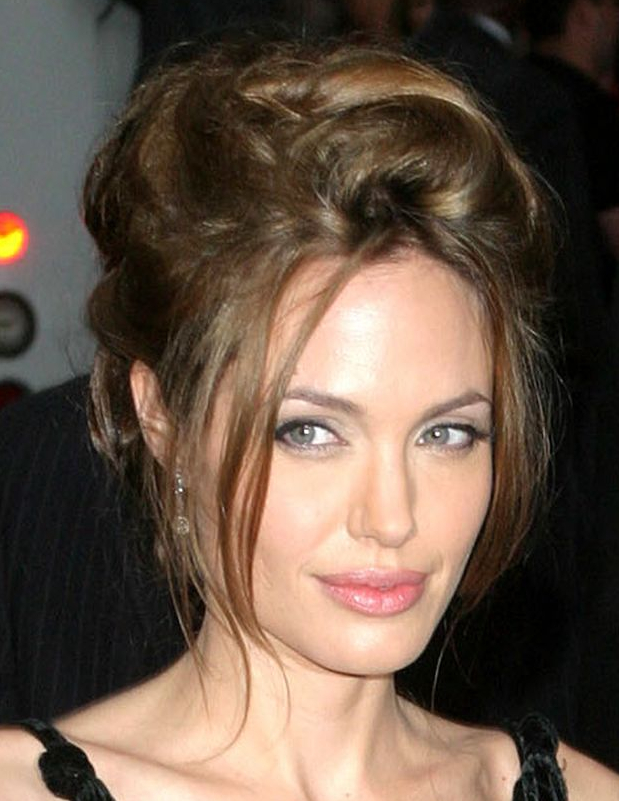
\includegraphics[width=0.16\textwidth]{Figures/chap1/angie_original.png}} &
			\subfloat{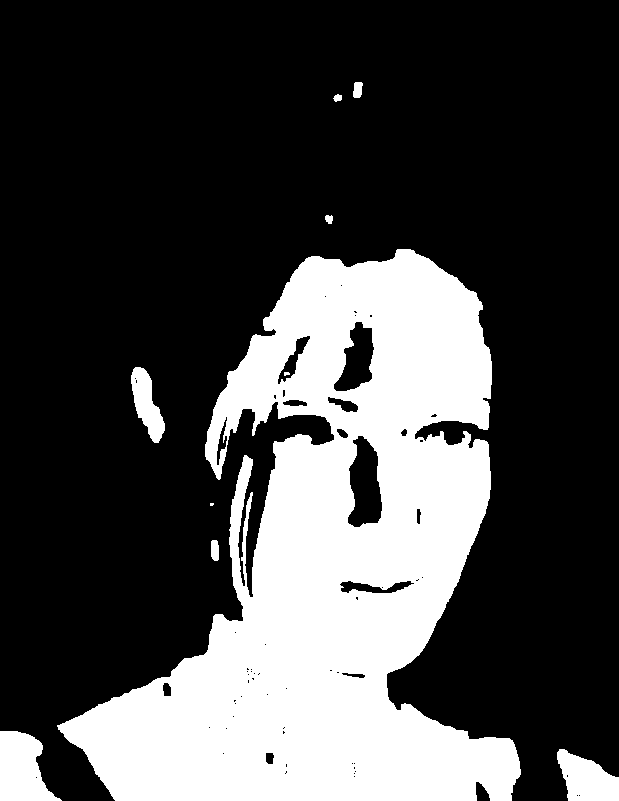
\includegraphics[width=0.16\textwidth]{Figures/chap1/EGGER_Segmentation_Nr_0.png}} &
			\subfloat{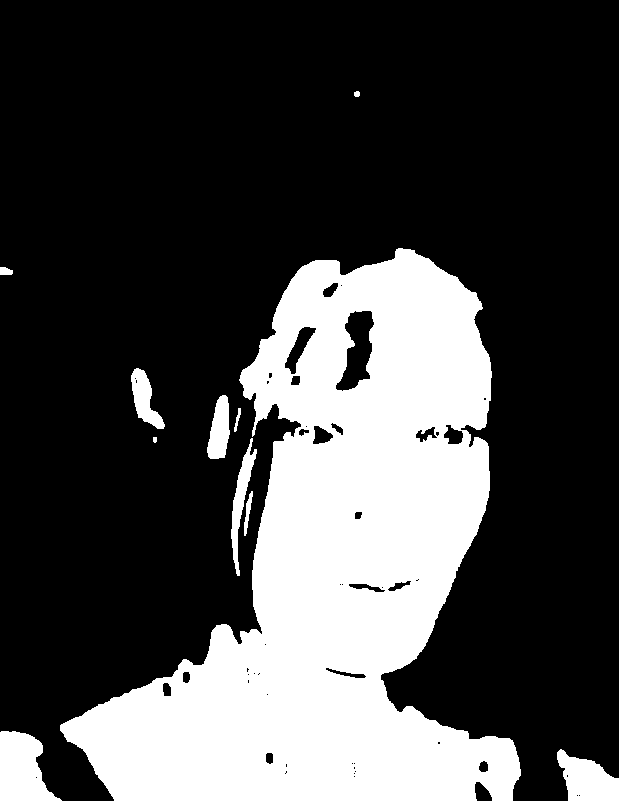
\includegraphics[width=0.16\textwidth]{Figures/chap1/EGGER_Segmentation_Nr_9.png}} &
			\subfloat{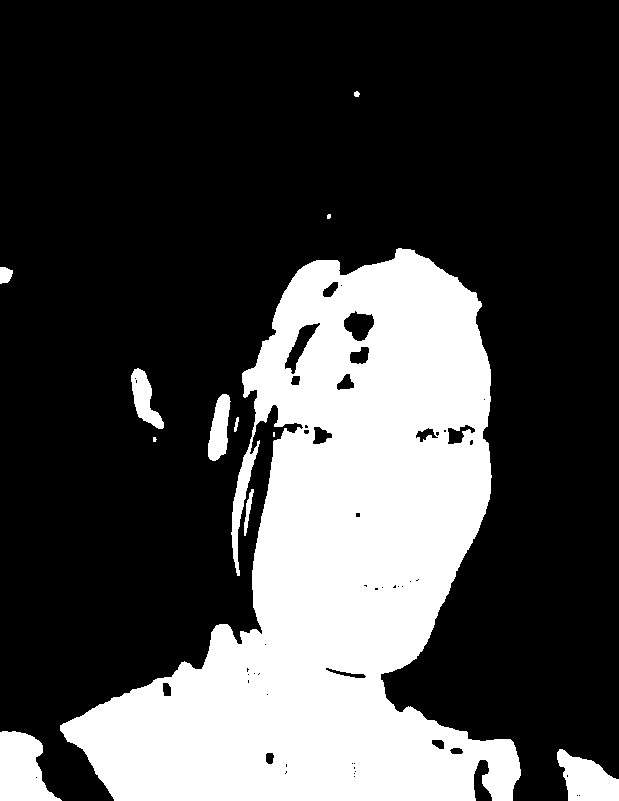
\includegraphics[width=0.16\textwidth]{Figures/chap1/EGGER_Segmentation_Nr_19.png}}&
			\subfloat{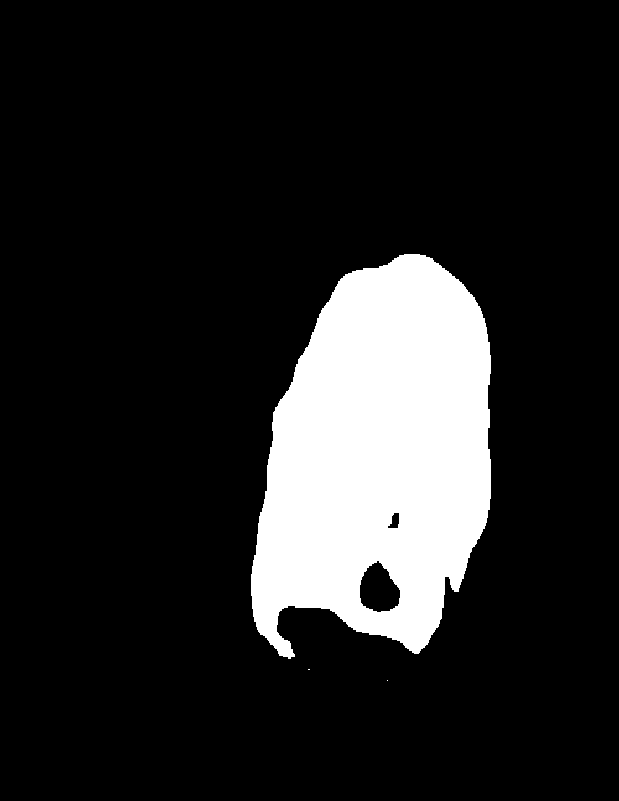
\includegraphics[width=0.16\textwidth]{Figures/chap1/angie_FCN.png}} \\
		\end{tabular}
	\end{center}
	\caption{This picture shows the development of the labels after 0, 10 and 20 iterations. Noticeable in this sample image are not only the eyes as mentioned before but also the shadow of the nose, which is first segmented as a background. Only after a certain number of iterations these errors are partially recognised and provided with the correct label.}
	\label{fig:iterations}
\end{figure}

\begin{figure}[H]
	\centering
	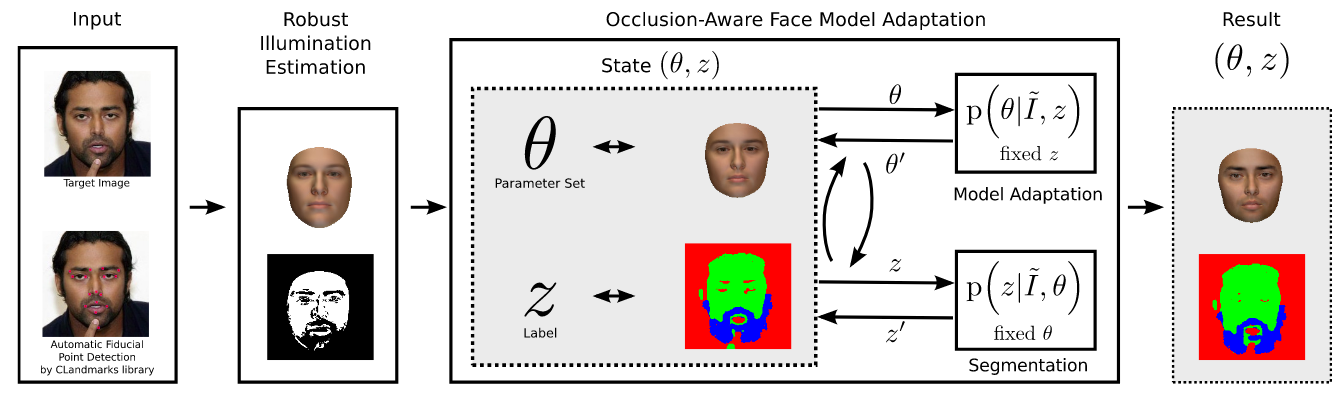
\includegraphics[width=1\linewidth]{Figures/chap1/EGGER's_method.png}
	\caption[Caption for LOF]{\footnotemark \  Algorithm overview: As input, the algorithm takes a target image and fiducial points. The external Clandmark library for automated fiducial point detection from still images [U\v ri\v c\' a\v r et al (2015) \cite{Uricar}] is used. The algorithm starts with an initial face model fit of our average face with a pose estimation. Then, a robust illumination estimation for initialisation of the segmentation labels z and the illumination settings is performed. For this task, a random sample consensus (RANSAC) algorithm is used. RANSAC methods estimate parameters of a mathematical model from a set of observed data that contains outliers. Then the face model and the segmentation are simultaneously adapted to the target image I. The result is a set of face model parameters $\Theta$ and a segmentation into face and non-face regions. The presented target image is from the LFW database (Huang et al (2007))}
	\label{fig:EGGER's_method}
\end{figure}

\footnotetext{Figure \ref{fig:EGGER's_method} is copied from Fig.4 of the "Occlusion-aware  3D  Morphable  Models and Illumination Prior for Face Image Analysis" paper of Egger et al. \cite{egger_paper}}

% Soll ich auch die 'stable illumination estimation' in ein chapter machen? Wenn ja, was ist das 'consensus set' ?

% The source for this table was this post: https://stackoverflow.com/questions/2771856/centering-text-horizontally-and-vertically-in-latex
% To add padding for the cell contents: https://tex.stackexchange.com/questions/31672/column-and-row-padding-in-tables
An approach using convolutional neural networks to segment occluded faces has already been described by \cite{SaitoEtAl}. The big difference to our approach is that multiple frames are needed for the final segmentation. Another approach of Morel-Forster et al \cite{MorelForster} uses random forests to detect facial-occlusions by hair. These are integrated into the fitting process in order to model uncertainty. Unlike us, Morel-Forster et al integrate the occlusion in the face likelihood of the evaluator.